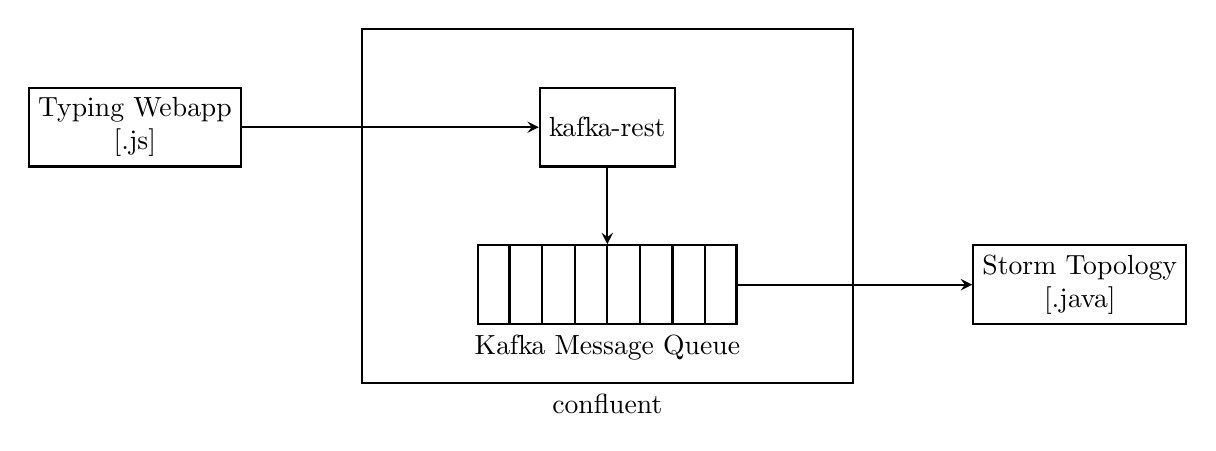
\begin{tikzpicture}[>=stealth]
	\usetikzlibrary{shapes}
  \node (webapp)			at (0,2) [rectangle, draw, minimum height=1cm,thick,align=center] {Typing Webapp \\ {[.js]}};
  \node (kafka)			at (6,0) [rectangle split, rectangle split parts=8, rectangle split horizontal, draw, minimum height=1cm,thick,align=center,label=below:Kafka Message Queue] {};
  \node (kafka-rest)			at (6,2) [rectangle, draw, minimum height=1cm,thick] {kafka-rest};
  \node (confluent)			at (6,1) [rectangle, draw, minimum height=4.5cm,thick,text width=6cm,align=center,label=below:confluent] {};
  \node (storm)			at (12,0) [rectangle, draw, minimum height=1cm,thick,align=center] {Storm Topology\\ {[.java]}};

		\path
		(webapp)					edge[->,thick] (kafka-rest)
		(kafka-rest)					edge[->,thick] (kafka)
		(kafka)					edge[->,thick] (storm);
\end{tikzpicture}
